\documentclass[12pt, a4paper, oneside]{ctexart}

\usepackage[table,svgnames]{xcolor}

\usepackage{graphicx,amsmath,amssymb,geometry,float}
\usepackage{pdfpages}

\usepackage{listings}
\usepackage{matlab-prettifier}

\usepackage{enumerate,enumitem}
\usepackage{autobreak}
\usepackage{breqn}

\geometry{left=2.5cm, right=2.5cm, top=2.5cm, bottom=2.5cm}

\usepackage{booktabs,array,tabularx}

\usepackage{fancyhdr}
\renewcommand{\headrulewidth}{0pt}
\pagestyle{fancy}
\fancyhf{}
\cfoot{\thepage}

\usepackage[font=footnotesize]{caption} 

\newtheorem{assumption}{假设}[section]

\CTEXsetup[name={,、\hspace{-1em}},number={\chinese{section}}]{section}

%\documentclass{standalone}

\usepackage{tikz}
\usetikzlibrary{arrows.meta, patterns, angles, calc, positioning}
\tikzset{ x=1cm, y=1cm, >=Latex, Ap/.style={draw, solid, <-, shorten <=2pt, angle radius=#1cm, angle eccentricity=1.1} }
\def\myR{1} \def\myangle{70}






\begin{document}
%\thispagestyle{empty}
% \begin{figure}[H]
%   \centering
%   \includegraphics[width=\textwidth]{pic/2022face.pdf}
% \end{figure}
\songti
\zihao{-4}
\title{波浪能最大输出功率优化设计\vspace{-3em}}
\date{}


\newpage
\setcounter{page}{1}
\maketitle
\author{\centerline{\kaishu 浙江大学\ \ 赵云鹏\ 何逸阳\ 闻人豪昱}}
\begin{abstract}

波浪能作为一种海洋可再生能源,在可再生能源产业中起着重要的作用。本文研究了一种波浪能转换装置,建立了由浮子和振子组成的动力学系统模型,并针对不同情况进行\textbf{解析解}和数值解的计算。此外,根据模型求解结果以最大化平均功率为目标获得相关参数的最优值,并对其做敏感度分析以获得参数的较优区间.

针对问题一、二,我们首先建立了浮子和振子一维垂荡运动的运动模型,并对二者分别进行受力分析得到运动方程。在阻尼系数恒定的情况下,方程为二阶常系数线性微分方程组,我们通过\textbf{拉普拉斯变换}的方式求得方程在像空间的解,再使用\textbf{Mathematica} 通过有理分式反演法进行逆变换得到方程的解。阻尼系数不恒定时,微分方程组包含非线性项,较难求出解析解。为了求解这个初值问题,我们在分析了方程的刚性后,选择使用隐式\textbf{Runge-Kutta}方法求得数值解。求得数值解后通过\textbf{辛普森法}积分计算功率,进而通过\textbf{下山单纯形法}以最大输出功率为目标对阻尼器的阻尼系数与幂指数进行优化。

针对问题三、四,在同时考虑垂荡的纵摇的情况下,运动的自由度增加至四个。我们对振子、浮子受力分析,进而得到三个受力方程、两个力矩方程,对应四个坐标以及一个内部力。由于该方程有许多非线性项,我们选择使用数值方法求解。同样在分析了方程的刚性后,我们选择使用五阶隐式\textbf{Runge-Kutta}方法固定步长求解,进而用\textbf{辛普森法}积分,最后用\textbf{下山单纯形法}优化。

随后我们通过查阅资料,对所用数值求解方法进行了粗略的精度分析,确定我们的数值算法精度为\textbf{四阶精度},并估计了所用步长下的求解误差,画出了此误差下各个参数最优的粗略范围。

最后,我们就不同大小的激励力振幅做了\textbf{敏感度分析},确定了适用此模型的海浪大小范围。






\noindent
\textbf{关键词 :} 波浪能利用;受迫耦合振动;拉普拉斯变换; Runge-Kutta法;下山单纯形法
\end{abstract}

\newpage
\section{问题重述}
\subsection{问题背景}
  波浪能作为一种海洋可再生能源,在可再生能源产业中起着重要的作用。本题中,一种波浪能装置利用波浪引起浮子与振子的相对运动,进而驱动阻尼器做功产生能量输出。具体需要解决如下四个问题。
\subsection{具体问题重述}
\textbf{第一问:}
问题一要求建立模型并求解问题。在给定波浪能装置运动结构,仅考虑浮子在竖直方向的垂荡运动的条件下,建立浮子与振子在波浪激励力作用下的运动模型。分别在阻尼系数恒定和阻尼系数与速度成幂次关系两种阻尼模式下,对初始位于平衡状态的浮子和振子应用运动模型进行求解,给出相应时刻的浮子与振子的速度与位移。



\textbf{第二问:}
问题二是问题一的优化问题,
浮子在波浪中仅作垂荡运动的条件下,分别对问题一的两种阻尼模式建立确定阻尼器最优阻尼系数的数学模型,以PTO平均输出功率最大为目标,对比例系数与幂指数进行优化,并计算最大输出功率及相应最优阻尼系数。

\textbf{第三问:}
问题三在问题一的基础上加装旋转阻尼器和转轴架,考虑浮子的垂荡和纵摇运动,要求建立浮子与振子同时在波浪激励力和波浪激励力矩作用下的运动模型。对于给定的阻尼系数,求解初始位于平衡状态下,不同时刻的浮子与振子的垂荡位移与速度和纵摇角位移与角速度。

\textbf{第四问:}
问题四是问题三的优化问题,在问题三的基础上建立确定直线阻尼器和旋转阻尼器最优阻尼系数的数学模型,以PTO平均输出功率最大为目标,对阻尼系数优化,并计算最大输出功率及相应最优阻尼系数。

\section{模型假设}
\begin{assumption}\label{asmp:watersurf}
水面近似保持静止(由于是微幅波,因此水面的上下波动不纳入考虑);
\end{assumption}
\begin{assumption}\label{asmp:output}
假设阻尼对外输出功率转化效率是常数(因此不妨设其为1,不纳入考虑);
\end{assumption}
\begin{assumption}\label{asmp:massdis}
假设振子质量均匀分布在圆柱体上,并忽略杆的粗细,因此可以把振子近似看成实心圆柱体;
\end{assumption}
\begin{assumption}\label{asmp:outsideinfl}
假设振子完全不与外界接触,只受重力和浮子的影响。同时忽略海风等对浮子的影响;
\end{assumption}
\begin{assumption}\label{asmp:prlforce}
不考虑浮子横向上受力(因为其对发电无影响,可通过锚定等方法消除);
\end{assumption}
\begin{assumption}\label{asmp:deform}
假设振子、杆以及浮子在受力时不产生形变。
\end{assumption}

\section{符号说明}
\begin{table}[H]
    \centering
    \caption{符号说明}
    \renewcommand{\arraystretch}{2}
    \begin{tabular*}{\textwidth}{c||l}%l左对齐,c居中,r右对齐,p指定列宽度
        \toprule[1.5mm]
        \Large{\textbf{符号}} & \Large{\textbf{说明}} \\\hline
        %\midrule[1.5pt]
        \(m_{v}\) & 振子质量 \\\hline
        \(m_{f}\) & 浮子质量 \\\hline
        \(k\) & 弹簧刚度\\\hline
        \(k_m\) & 扭转弹簧刚度\\\hline
        \(\nu\) & 阻尼器的阻尼系数\\\hline
        \(m_a\) & 垂荡附加质量\\\hline
        \(I_a\) & 纵摇附加转动惯量\\\hline
        \(\mu\) & 垂荡兴波阻尼系数\\\hline
        \(\mu_m\) & 纵摇兴波阻尼系数\\\hline
        \(F\) &垂荡波浪激励力\\\hline
        \(L\) &纵摇激励力矩\\\hline
        \(r\) & 静水恢复力系数\\\hline
        \(r_m\) & 静水恢复力矩系数\\\hline
        \(t_f\) & 迭代终止时间(末时刻)\\\hline
        \bottomrule[1mm]
    \end{tabular*}
\end{table}

\section{问题分析}
\subsection{问题一分析}
由于题目要求只考虑振子和浮子在竖直方向上的运动,所以这是一个一维二体动力学问题的求解。我们对浮子和振子分别进行受力分析,再通过牛顿第二定律建立运动方程。因为初始状态固定(平衡于水中),外力形式和相互作用力形式已知,我们通过牛顿运动方程来确定任意时刻两物体的运动状态。
\begin{enumerate}
    \item 阻尼系数为常数:方程为二阶常系数线性微分方程组,可以通过拉普拉斯变换的方式求得方程的解析解,进而确定任意时刻浮子和振子的运动状态。
    \item 阻尼系数与浮子和振子的相对速度的绝对值的幂成正比:方程为非线性方程,不易求得解析解。分析得出方程的刚性较大,因此我们通过5阶隐式Runge-Kutta法固定步长对模型进行求解。
\end{enumerate}

\subsection{问题二分析}
浮子和振子的垂荡在固定频率的受迫力作用下会趋于稳定,因此我们计算在稳定状态下功率输出的最优解。
\begin{enumerate}
    \item 在第一小问中,我们使用复振幅法解析地求出了浮子和振子的稳定运动情况,并计算得到了平均输出功率与阻尼系数$\nu$的关系。通过Mathematica进行求导得到阻尼系数的最优值。
    \item 在第二小问中,我们选择使用复合Simpson方法进行数值积分得到平均功率。在对各个参数下的平均功率作图以及解析分析后,我们发现其局部最优解即全局最优解,进而采用下山单纯形法进行优化求解。
\end{enumerate}


\subsection{问题三分析}
由于水平方向的运动对输出功率没有影响,可以不纳入考虑,因此浮子和振子的运动系统共有四个自由度。我们对振子、浮子受力分析,进而获得三个受力方程、两个力矩方程,对应四个坐标以及一个内部力。由于方程具有许多非线性项,求解变得十分困难,几乎无法用解析方式得到结果。因此我们直接采用数值方法。同样由于方程刚性较大,我们通过5阶隐式Runge-Kutta法固定步长求解。

\subsection{问题四分析}
同问题二第二小问,我们通过数值积分的方法求得平均功率,并以最大平均功率为目标对两个阻尼系数进行优化。同样,我们发现局部最优解即为全局最优解,进而采用下山单纯形法进行优化求解。

\section{模型建立}

\subsection{仅考虑垂荡运动的模型}
\subsubsection{变量、符号说明}
\begin{table}[H]
    \centering
    \caption{变量说明}
    \renewcommand{\arraystretch}{2}
    \begin{tabular*}{\textwidth}{c|l}%l左对齐,c居中,r右对齐,p指定列宽度
        \toprule[0.5mm]
        \Large{\textbf{变量}} & \Large{\textbf{说明}} \\\hline
        \bottomrule[0.3mm]
        \(x_{v}\) & 振子的竖直偏移平衡位置的位移,正方向向上 \\\hline
        \(x_{f}\) & 浮子的竖直偏移平衡位置的位移,正方向向上 \\\hline
        \(P\) & 瞬时输出功率 \\\hline
        \(Pa\) & 平均输出功率 \\\hline
    \end{tabular*}
\end{table}
\subsubsection{受力分析}
对振子和浮子分别做受力分析,结果如下图所示。
\begin{figure}[!ht]
    \centering
    \begin{minipage}[t]{0.45\textwidth}
        \begin{tikzpicture}
            \draw (-2,-1.2) rectangle (2,1.2);
            \fill (0,0) circle (2pt) node[right]{振子};
            \draw[->,very thick] (0,0) -- (0,-1.8) node[right]{$\boldsymbol{f_\nu}$};
            \draw[->,very thick] (0,0) -- (0,-2.5) node[left]{$\boldsymbol{f_k}=-k(x_v-x_f)$};
        \end{tikzpicture}
        \caption{振子垂荡受力分析}
        \label{fig:vertv}
        
    \end{minipage}
    \begin{minipage}[t]{0.45\textwidth}
        \begin{tikzpicture}
        \draw (-3,-1.5) rectangle (3,1.5);
        \draw (-3,-1.5) -- (0,-3);
        \draw (3,-1.5) -- (0,-3);
        \fill (0,0) circle (2pt) node[right]{浮子};
        \draw[->,very thick] (0,0) -- (0,2.2) node[right]{$\boldsymbol{-f_\nu}$};
        \draw[->,very thick] (0,0) -- (0,3.5) node[right]{$\boldsymbol{F}$};
        \draw[->,ultra thick] (0,0) -- (0,-2.1) node[] at (1.15,-1.78){$\boldsymbol{f_r}=-r x_f$};
        \draw[->,ultra thick] (0,0) -- (0,-3.2) node[right]{$\boldsymbol{f_\mu}=-\mu\dot{x}_f$};
        \draw (1,-1.5)arc[start angle=0, end angle=180,  radius=1];
        \draw[->,very thick] (0,0) -- (0,3.0) node[left]{$\boldsymbol{-f_k}$};
    \end{tikzpicture}
        \caption{浮子垂荡受力分析}
        \label{fig:vertf}
    \end{minipage}
    
\end{figure}



\begin{figure}[!ht]
    \centering
    \scalebox{1.0}{
    
    }
\end{figure}

\textbf{振子受力分析}

对振子而言,平衡位置处弹簧的弹力与浮子的重力保持平衡,所以在偏移平衡位置后所受的合力为弹簧弹力的改变量$f_k=-k(x_v-x_f)$以及阻尼器的阻力$f_\nu$,
由牛顿第二定律得出振子运动方程:
\begin{equation}
    m_v\ddot x_v=-k (x_v- x_f)-\boldsymbol{f_\nu}
\end{equation}

\textbf{浮子受力分析}

对浮子而言,同样平衡位置的浮力与重力保持平衡,偏移平衡位置后所受的合力为
\begin{equation}  
             \begin{cases}
            \text{垂荡波浪激励力}\quad F\\  
            \text{弹簧的弹力变化量}\quad -f_k=k(x_v-x_f)\\  
            \text{阻尼器的阻力}\quad -f_\nu\\
            \text{垂荡兴波阻尼力}\quad f_\mu=-\mu \dot x_f\\
            \text{静水恢复力}\quad f_r
             \end{cases}  
\end{equation} 
%垂荡波浪激励力$F$,弹簧的弹力变化量$-f_k=k(x_v-x_f)$,阻尼器的阻力$-f_\nu$,垂荡兴波阻尼力$f_\mu=-\mu \dot x_f$,静水恢复力$f_r$

经计算,浮子漏出水面高度1m,水下圆柱部分2m,由后续求解可知浮子振幅小于1m,静水恢复力在线性区间(圆柱区间)。因此静水恢复力有以下形式:
$$f_r=-r x_f$$其中 $$r=\rho g \pi R^2 $$


此外,由于推动浮体做摇荡运动的力不仅要推动浮体运动,还要推动浮体
周围的流体运动,因而要使浮体在海水中获得加速度,需要施加额外的力,对应牛顿方程中惯性质量的增加$(m_a)$。可得:
$$(m_f+m_a)\ddot x_f=k (x_v- x_f)+\boldsymbol{f_\nu}-\mu\dot x_f+\boldsymbol F-r x_f$$

综上,由题目要求得到以下IVP(初值问题):
\begin{equation}
\label{equ:ivp1}
 \begin{aligned}
  \begin{cases}
    & m_v\ddot x_v=-k (x_v- x_f)-\boldsymbol{f_\nu}\\
    &(m_f+m_a)\ddot x_f=k (x_v- x_f)+\boldsymbol{f_\nu}-\mu\dot x_f+\boldsymbol F-r x_f\\
    &x_v(0)=x_f(0)=\dot x_v(0)=\dot x_f(0)=0
  \end{cases}
 \end{aligned}
\end{equation}

\subsubsection{功率计算}
对于功率的计算,根据题目描述,我们知道功率输出全部来自阻尼器。由假设\ref{asmp:output},我们得到功率计算公式:
\begin{equation}
    P=f_\nu (\dot x_v-\dot x_f)
\end{equation}
由于系统稳定时处于振荡状态,因此我们应当求其平均输出功率:
\begin{equation}
    Pa=\frac1{t_f}\int_0^{t_f}P(t)dt
\end{equation}





\subsection{考虑垂荡和纵摇运动的模型}
\subsubsection{变量、符号说明}
\begin{table}[H]
    \centering
    \caption{变量、符号说明}
    \renewcommand{\arraystretch}{2}
    \begin{tabular*}{\textwidth}{c|l}%l左对齐,c居中,r右对齐,p指定列宽度
        \toprule[0.5mm]
        \large{\textbf{符号}} & \large{\textbf{说明}} \\\hline
        \bottomrule[0.3mm]
        \(x_{v}\) & 振子与浮子的相对位移,正方向向外(与前文不同) \\\hline
        \(x_{f}\) & 浮子的竖直偏移平衡位置的位移,正方向向上 \\\hline
        \(\theta_{v}\) & 振子与浮子圆柱轴线的相对夹角,顺时针为正 \\\hline
        \(\theta_{f}\) & 浮子圆柱轴线与竖直方向夹角,顺时针为正 \\\hline
        \(\overrightarrow{R}\) & 振子的位矢 \\\hline
        \(\overrightarrow{i}\) & 竖直向上基矢 \\\hline
        \(\overrightarrow{e_r}\) & 中轴轴向基矢 \\\hline
        \(\overrightarrow{e_\theta}\) & 中轴法向基矢 \\\hline
        \(I_v\) & 振子对转轴的转动惯量(与$x_v$有关) \\\hline
        \(I_f\) & 浮子对转轴的转动惯量(常数) \\\hline
    \end{tabular*}
\end{table}
\subsubsection{加速度分析}
对振子建立牛顿第二定律方程,需要计算振子的加速度。设振子的位矢为\(\overrightarrow{R}\),有:
$$\overrightarrow{R}=\overrightarrow{x_f}+\overrightarrow{x_v}=x_f\overrightarrow{i}+x_v\overrightarrow{e_r}$$
由几何关系,我们有:
$$\dot{\overrightarrow{e_r}}=(\dot \theta_f+\dot \theta_v)\overrightarrow{e_\theta}$$
$$\dot{\overrightarrow{e_\theta}}=-(\dot \theta_f+\dot \theta_v)\overrightarrow{e_r}$$
$$\overrightarrow{i}=\cos(\theta_f+\theta_v)\overrightarrow{e_r}-\sin(\theta_f+\theta_v)\overrightarrow{e_\theta}$$
因此振子的速度:
\begin{align*}
    \frac{d \overrightarrow{R}}{d t}&=\dot x_f \overrightarrow{i}+\dot x_v \overrightarrow{e_r}+x_v \dot{\overrightarrow{e_r}}\\
    &=\dot x_f \overrightarrow{i}+\dot x_v\overrightarrow{e_r}+x_v (\dot \theta_f+\dot \theta_v)\overrightarrow{e_\theta}
\end{align*}
振子的加速度:
\begin{align*}
     \frac{d^2 \overrightarrow{R}}{d t^2}&=\ddot x_f \overrightarrow{i}+\ddot x_v \overrightarrow{e_r}+\dot{x_v} (\dot \theta_f+\dot \theta_v)\overrightarrow{e_\theta}+\dot{x_v} (\dot \theta_f+\dot \theta_v)\overrightarrow{e_\theta}+{x_v} (\ddot \theta_f+\ddot \theta_v)\overrightarrow{e_\theta}-x_v (\dot \theta_f+\dot \theta_v)^2\overrightarrow{e_r}\\
     &=\left(\ddot x_f\cos(\theta_f+\theta_v)+\ddot x_v-x_v (\dot \theta_f+\dot \theta_v)^2\right) \overrightarrow{e_r}
     \\&\qquad +\left( -\ddot x_f\sin(\theta_f+\theta_v)+2\dot{x_v} (\dot \theta_f+\dot \theta_v) +{x_v} (\ddot \theta_f+\ddot \theta_v)\right)\overrightarrow{e_\theta}
\end{align*}
\subsubsection{受力分析}
在同时考虑垂荡和纵摇运动情况下,振子和浮子受力分析如图\ref{fig:force}所示.
\begin{figure}[H]
    \centering
    \begin{minipage}[t]{0.55\textwidth}
        \begin{tikzpicture}[scale=0.8]
            %\draw [step=1cm] (-6,-7) grid (6,7);
            \draw[domain=-6:-2.7,smooth] plot(\x,{1+0.3*sin(4*\x r)}) node[left=7pt]{水面};
           \draw[domain=4:6,smooth] plot(\x,{1+0.3*sin(4*\x r)})node[above=1pt]{水面};
           \draw[rotate=-30,thick] (-3,-1) -- (0,-3);
           \draw[rotate=-30,thick] (3,-1) -- (0,-3);
           \draw[rotate=-30,thick] (-3,-1) rectangle (3,4.6);
           \draw[->,ultra thick] (-1,-1.75) -- (-1,5) node[left] {$\boldsymbol{F}=f\cos{\omega t}$};
           \draw[->,ultra thick] (-1,-1.75) -- (-1,-3.25) node[] at (0.2,-3) {$\boldsymbol{f_a}=-m_a\ddot{x}_f$};
           \draw[->,ultra thick] (-1,-1.75) -- (-1,-4.75) node[] at (0.2,-4.5) {$\boldsymbol{f_\mu}=-\mu\dot{x}_f$};   
           \draw[->,ultra thick] (-1,-1.75) -- (-1,-5.75) node[] at (0.2,-5.5) {$\boldsymbol{f_r}=-r x_f$};           
           \fill (-1,-1.75) circle (2pt) ;
           
           \draw[thick] (0.4,-1.4)arc[start angle=-30, end angle=150, radius=1];
           %\draw[very thick] (0.4,-1.4) -- (-1.36,-0.4);
           \draw[densely dotted] (-0.12,0.06) -- (1.8,2);
           \draw[densely dotted] (0.17,-0.1) -- (2,1.8);
           \draw[densely dotted] (1.8,2) -- (2,1.8);
           \draw[densely dotted] (0,1) -- (1,2) -- (2,1) -- (1,0) -- (0,1);
            \fill (-0.2,-0.2) circle (2pt);
            \draw[->,ultra thick] (-0.2,-0.2) -- (0.75,0.75) node[] at (2.0,1.5) {$\boldsymbol{f_k}$} ;
            \draw[->,ultra thick] (-0.2,-0.2) -- (1.75,1.75) node[] at (1.3,-0.2) {$\boldsymbol{f_\nu}=\nu \dot{x}_v$};
            \draw[->,ultra thick] (-0.2,-0.2) -- (-4,3.6) node[above] {$\boldsymbol{F_1}$};
            \draw[->,thick] (-0.2,-0.2) -- (-0.2,3.6);
            \draw[->,thick] (-0.2,-0.2) -- (-0.2,0.75);
            \draw[->,thick] (-0.2,-0.2) -- (-0.2,1.75);
            \draw [dashed] (-4,3.6)--(-0.2,3.6);
            \draw (-0.4,3.6)--(-0.4,3.4)--(-0.2,3.4);
            \draw [dashed] (0.75,0.75)--(-0.2,0.75);
            \draw [dashed] (1.75,1.75)--(-0.2,1.75);
            \draw (-0.2,0.6)--(-0.05,0.6)--(-0.05,0.75);
            \draw (-0.2,1.6)--(-0.05,1.6)--(-0.05,1.75);
            \draw[dash dot] (-1,-1.75) -- (3,6);
            \draw[dash dot] (-0.2,-0.2) -- (4,4);
            \draw[dash dot] (-0.2,0) -- (-0.2,5);
            
            \draw[loosely dashed,->] (1.6,3.09375)arc[start angle=62.7, end angle=46.5,  radius=3.71] node[] at (2.3,3) {$\theta_v$};
            \draw[loosely dashed,<-] (1.25,2.6)arc[start angle=62.7, end angle=91.5,  radius=2.88] node[] at (0.5,3.1) {$\theta_f$};
        \end{tikzpicture}
        
    \end{minipage}
    \begin{minipage}[t]{0.35\textwidth}
        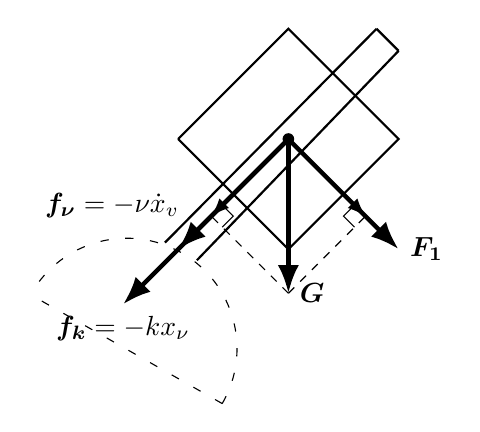
\begin{tikzpicture}[scale=1.4]
        %\draw [step=1cm] (-6,-7) grid (6,7);

       \draw[loosely dashed] (0.4,-1.4)arc[start angle=-30, end angle=150, radius=1];
       \draw[loosely dashed] (0.4,-1.4) -- (-1.36,-0.4);
       \draw[thick] (-0.12,0.06) -- (1.8,2);
       \draw[thick] (0.17,-0.1) -- (2,1.8);
       \draw[thick] (1.8,2) -- (2,1.8);
       \draw[thick] (0,1) -- (1,2) -- (2,1) -- (1,0) -- (0,1);
        \fill (1,1) circle(1.5pt);
        \draw[->,thick] (1,1) -- (0.3,0.3);
        \draw[->,ultra thick] (1,1) -- (0,0) node[] at (-0.6,.4)  {$\boldsymbol{f_\nu}=-\nu \dot{x}_v$};
        \draw[->,ultra thick] (1,1) -- (-0.5,-0.5) node[below] {$\boldsymbol{f_k}=-k x_\nu$};
        \draw[->,ultra thick] (1,1) -- (2,0) node[right] {$\boldsymbol{F_1}$};
        \draw[->,thick] (1,1) -- (1.7,0.3);
        \draw[->,ultra thick] (1,1) -- (1,-0.4) node[right] {$\boldsymbol{G}$};
        \draw[dashed] (1,-0.4) -- (0.3,0.3);
        \draw[dashed] (1,-0.4) -- (1.7,0.3);
        \draw (0.4,0.2) -- (0.5,0.3) -- (0.4,0.4);
        \draw (1.6,0.2) -- (1.5,0.3) -- (1.6,0.4);
    \end{tikzpicture}
    \end{minipage}
    \caption{振子、浮子受力分析图}
    \label{fig:force}
\end{figure}
\textbf{振子受力分析}

与前文不同,由于$x_v$并非从平衡位置开始,因此振子的重力项需单独考虑,我们设
\begin{equation}  
             \begin{cases}
            \text{振子重力}\quad G\\  
            \text{弹簧弹力}\quad f_k=-k x_\nu\\  
            \text{阻尼力}\quad f_\nu=-\nu \dot x_v\\
            \text{振子与浮子垂直于中轴方向的相互作用力}\quad F_1\\
             \end{cases}  
\end{equation} 
%振子的重力为$G$,弹簧弹力为$f_k=-k x_\nu$,阻尼力为$f_\nu=-\nu \dot x_v$。设振子与浮子垂直于中轴方向的相互作用力为$F_1$,
各力方向如图\ref{fig:force}所示。

由前文计算$\overrightarrow{e_r}$方向加速度可得

沿中轴方向运动方程:
$$m_v\left(\ddot x_f\cos(\theta_f+\theta_v)+\ddot x_v-x_v (\dot \theta_f+\dot \theta_v)^2\right) =-k (x_v-l)-\nu\dot x_v-m_v g\cos(\theta_v+\theta_f)$$

垂直中轴方向运动方程:
$$m_v\left( -\ddot x_f\sin(\theta_f+\theta_v)+2\dot{x_v} (\dot \theta_f+\dot \theta_v) +{x_v} (\ddot \theta_f+\ddot \theta_v)\right)=F_1+m_v g\sin(\theta_f+\theta_v)$$

\textbf{浮子受力分析}

对于浮子,只考虑竖直方向的垂荡运动。我们将振子重力项并入弹簧恢复力,即以$l-m_v g/k$为弹簧平衡位置计算弹簧弹力分力$f_k=k(x_v-l+m_v g /k)\cos(\theta_v+\theta_f)$,浮子重力项并入静水恢复力$f_r=-r x_f$中,综上得竖直方向力为
%竖直方向还受力振子作用力分力$F_1\sin(\theta_v+\theta_f)$,阻尼力分力$f_\nu=\nu x_v\cos(\theta_v+\theta_f)$,兴波阻尼力$f_\mu=-\mu \dot x_f$,附加惯性力$fa=-m_a\ddot x_f$,波浪激励力$F=f \cos (\omega t)$。
\begin{equation}  
             \begin{cases}
             \text{弹簧弹力分力}\quad f_k=k(x_v-l+m_v g /k)\cos(\theta_v+\theta_f)\\  
             \text{静水恢复力}\quad f_r=-r x_f\\  
            \text{振子作用力分力}\quad F_1\sin(\theta_v+\theta_f)\\  
            \text{阻尼力分力}\quad f_\nu=\nu x_v\cos(\theta_v+\theta_f)\\
            \text{兴波阻尼力}\quad f_\mu=-\mu \dot x_f\\
            \text{附加惯性力}\quad fa=-m_a\ddot x_f\\
            \text{波浪激励力}\quad F=f \cos (\omega t)\\
             \end{cases}  
\end{equation} 

浮子竖直方向运动方程:
$$m_f\ddot x_f=k(x_v -l+m_vg/k)\cos(\theta_v+\theta_f)-rx_f+F_1\sin(\theta_v+\theta_f)+\nu\dot x_v\cos(\theta_v+\theta_f)-\mu\dot x_f-m_a\ddot x_f+f \cos (\omega t)$$
\subsubsection{力矩分析}
\textbf{转动惯量计算}

首先计算振子对转轴的转动惯量,均匀圆柱体对经过质心直径的转动惯量为:
$$\frac{m_v r_v^2}{4}+\frac{m_v h_v^2}{12}$$

由平行轴定理可得振子的转动惯量为$(m_v=2433,r_v=0.5,h_v=0.5)$:
$$I_v=\frac{m_v r^2}{4}+\frac{m_v h^2}{12}+m_v x_v^2$$

随后我们计算浮子外壳对转轴的转动惯量。圆柱、圆锥的高度$H_1=3,H_2=0.8$,半径$R=1$,圆柱、圆锥的质量分别为$m_1$,$m_2$($m1+m2=m_f=4866$),令$L=\sqrt{R^2+H_2^2}$为圆锥母线长度,则有:
$$m_1=\frac{2\pi RH_1}{\pi R L+2\pi RH_1}m_f$$
$$m_2=\frac{\pi R L}{\pi R L+2\pi RH_1}m_f$$
对圆锥和圆柱壳简单积分可得:
$$I_f=\frac{m_1 R^2}{2}+\frac{m_1 H_1^2}{3}+\frac{m_2H_2^2}{6}+\frac{m_2R^2}{4}$$
\textbf{振子力矩分析}

如图\ref{fig:moment}所示
\begin{figure}[H]
    \centering
    \scalebox{0.7}{
    \begin{tikzpicture}
        %\draw [step=1cm] (-6,-7) grid (6,7);
        \draw[domain=-6:-2.7,smooth] plot(\x,{1+0.3*sin(4*\x r)}) node[left=7pt]{水面};
       \draw[domain=4:6,smooth] plot(\x,{1+0.3*sin(4*\x r)})node[above=5pt]{水面};
       \draw[thick] (0.4,-1.4)arc[start angle=-30, end angle=150, radius=1];
       \draw[rotate=-30,thick] (-3,-1) -- (0,-3);
       \draw[rotate=-30,thick] (3,-1) -- (0,-3);
       \draw[rotate=-30,thick] (-3,-1) rectangle (3,4.6);
       %\draw[ultra thick] (0,0) -- (2,2);
       \draw[thick] (-0.12,0.06) -- (1.8,2);
       \draw[thick] (0.17,-0.1) -- (2,1.8);
       \draw[thick] (1.8,2) -- (2,1.8);
       \draw[thick] (0,1) -- (1,2) -- (2,1) -- (1,0) -- (0,1);
       \draw[->,ultra thick] (-1,6)arc[start angle=100, end angle=30,  radius=6.08] node[left=1.5cm][above=1.5cm]{$\boldsymbol{M_d}=L \cos{\omega t}$};
       \draw[->,ultra thick] (3,2)arc[start angle=10, end angle=100,  radius=1.4] node[above=1.5pt]{$\boldsymbol{M_\nu}=-\nu_m \dot{\theta}_v$};
       \draw[->,ultra thick] (2.5,1.5)arc[start angle=10, end angle=90,  radius=1.6] node[below=0.18cm]{$\boldsymbol{M_k}=-k_m \theta_v$};
       \draw[<-,ultra thick] (2.8,1.7)arc[start angle=10, end angle=90,  radius=1.6] node[] at (3,1.4){$\boldsymbol{M_g}$};
       
       \draw[->,ultra thick] (-3.5,-0.5)arc[start angle=190, end angle=290,  radius=3.2] node[]at (-0.2,-3.3) {$\boldsymbol{M_\mu}=-\mu_m \dot{\theta}_f$};
       \draw[->,ultra thick] (-4,-1)arc[start angle=190, end angle=295,  radius=3.5] node[] at(-0.5,-4.2) {$\mathbf{M_a}=-I_a \ddot{\theta}_f$};
       \draw[->,ultra thick] (-4.5,-1.5)arc[start angle=190, end angle=290,  radius=4] node[]at(-0.5,-5.2){$\mathbf{M_r}=-r_m \theta_f$};
       
       \draw[->,ultra thick] (-1.3,0)arc[start angle=150, end angle=-40,  radius=1.2] node[]at(2,-0.3){\small $\boldsymbol{-M_\nu}=\nu_m \dot{\theta}_v$};
       
       \draw[->,ultra thick] (0.15,-1.6)arc[start angle=290, end angle=180,  radius=1.1] node[]at(-0.5,-1.9){$\mathbf{-M_k}=k_m \theta_v$};
    \end{tikzpicture}
    }
    \caption{振子、浮子力矩分析}
    \label{fig:moment}
\end{figure}


振子的力矩来源有三个,分别为
\begin{equation}  
             \begin{cases}
            \text{扭转弹簧的扭矩}\quad M_k=-k_m\theta_v\\  
            \text{旋转阻尼器的扭矩}\quad M_\nu=-\nu_m \dot\theta_v\\  
            \text{振子重力力矩}\quad M_g=m_v g x_v \sin(\theta_v+\theta_f)
             \end{cases}  
\end{equation} 
%扭转弹簧的扭矩$M_k=-k_m\theta_v$,旋转阻尼器的扭矩$M_\nu=-\nu_m \dot\theta_v$,以及振子重力力矩$M_g=m_v g x_v \sin(\theta_v+\theta_f)$,

由此可得转动方程:
$$-\nu_m\dot\theta_v-k_m\theta_v+m_v g x_v\sin(\theta_v+\theta_f)=I_v (\ddot\theta_v+\ddot\theta_f)$$

\textbf{浮子力矩分析}

浮子的力矩来源分别为
\begin{equation}  
             \begin{cases}
            \text{扭转弹簧的扭矩}\quad -M_k=k_m\theta_v\\  
            \text{旋转阻尼器的扭矩}\quad -M_\nu=\nu_m \dot\theta_v\\  
            \text{静水恢复力矩(包含重力力矩)}\quad Mr=-r_m \theta_f\\
            \text{兴波阻尼力矩} \quad M_\mu=-\mu_m \dot \theta_f\\
            \text{附加惯性力矩} \quad M_a=-Ia\ddot\theta_f\\
            \text{波浪激励力矩} \quad M_d=L\cos(\omega t)
             \end{cases}  
\end{equation} 
%扭转弹簧的扭矩$-M_k=k_m\theta_v$,旋转阻尼器的扭矩$-M_\nu=\nu_m \dot\theta_v$,静水恢复力矩(包含重力力矩)$Mr=-r_m \theta_f$,兴波阻尼力矩$M_\mu=-\mu_m \dot \theta_f$,附加惯性力矩$M_a=-Ia\ddot\theta_f$,波浪激励力矩$M_d=L\cos(\omega t)$

由此可得转动方程:
$$k_m\theta_v+\nu_m\dot\theta_v-r_m \theta_f-\mu_m \dot\theta_f-I_a\ddot\theta_f+L\cos(\omega t)=I_f\ddot\theta_f$$

\subsubsection{模型状态方程}
综上,由题给初始条件可得$x_v$、$x_f$、$\theta_v$、$\theta_f$、$F_1$所满足的IVP为
\begin{equation}
\label{equ:ivp2}
 \begin{aligned}
  \begin{cases}
    & m_v\left(\ddot x_f\cos(\theta_f+\theta_v)+\ddot x_v-x_v (\dot \theta_f+\dot \theta_v)^2\right) =-k (x_v-l)-\nu\dot x_v-m_v g\cos(\theta_v+\theta_f)\\
    &m_v\left( -\ddot x_f\sin(\theta_f+\theta_v)+2\dot{x_v} (\dot \theta_f+\dot \theta_v) +{x_v} (\ddot \theta_f+\ddot \theta_v)\right)=F_1+m_v g\sin(\theta_f+\theta_v)\\
    &
    \begin{aligned}
     m_f\ddot x_f=&k(x_v -l+m_v g/k)\cos(\theta_v+\theta_f)-r x_f+F_1\sin(\theta_v+\theta_f)\\
     &+\nu\dot x_v\cos(\theta_v+\theta_f)-\mu\dot x_f-m_a\ddot x_f+f \cos (\omega t)
    \end{aligned}\\
    &-\nu_m\dot\theta_v-k_m\theta_v+m_v g x_v\sin(\theta_v+\theta_f)=I_v (\ddot\theta_v+\ddot\theta_f)\\
    &k_m\theta_v+\nu_m\dot\theta_v-r_m \theta_f-\mu_m \dot\theta_f-I_a\ddot\theta_f+L\cos(\omega t)=I_f\ddot\theta_f\\
    &\begin{aligned}
    &x_v(0)=l-m_vg/k,\\ 
    &x_f(0)=\dot x_v(0)=\dot x_f(0)=0\\
    &\theta_v(0)=\theta_f(0)=\dot\theta_v(0)=\dot\theta_f(0)=0
    \end{aligned}
  \end{cases}
 \end{aligned}
\end{equation}
\section{模型求解}
\subsection{问题一的求解}
\subsubsection{第一小问}
在该小问中,\(\boldsymbol{f_\nu}\)为线性项$\nu(\dot x_v-\dot x_f)$,激励力$\boldsymbol F=f\cos(\omega t)$,代入式(\ref{equ:ivp1})得到二阶线性常系数微分方程组:
\begin{equation}
 \begin{aligned}
  \begin{cases}
       & m_v\ddot x_v=-k (x_v- x_f)-\nu(\dot x_v-\dot x_f)\\
       &(m_f+m_a)\ddot x_f=k (x_v- x_f)+\nu(\dot x_v-\dot x_f)-\mu\dot x_f-r x_f+f\cos(\omega t)\\
  \end{cases}
 \end{aligned}
\end{equation}


对方程进行拉普拉斯变换得到

\begin{dmath}
  \begin{cases}
       & m_v p^2\bar x_v(p)=-k(\bar x_v(p)- \bar x_f(p))-\nu p (\bar x_v(p)-\bar x_f(p))\\
    &(m_f+m_a)p^2\bar x_f(p)=k (\bar x_v(p)- \bar x_f(p))+\nu p (\bar x_v(p)-\bar x_f(p))-\mu p \bar x_f-r \bar x_f(p)+f \frac{p}{p^2+\omega^2}
  \end{cases}
\end{dmath}
解得 
\begin{equation}
 \begin{aligned}
  \begin{cases}
       & \bar x_f(p)=\frac{f p \left(k+m_v p^2+p v\right)}{\left(p^2+w^2\right) \left(\left(k+m_v p^2+p v\right) \left(k+p^2 (m_a+m_f)+p u+p v+r\right)-(k+p v)^2\right)}\\
    &\bar x_v(p)=\frac{f p (k+p v)}{\left(p^2+w^2\right) \left(k m_a p^2+k m_f p^2+k m_v p^2+k p u+k r+m_a m_v p^4+m_a p^3 v+m_f m_v p^4+m_f p^3 v+m_v p^3 u+m_v p^3 v+m_v p^2 r+p^2 u v+p r v\right)}
  \end{cases}
 \end{aligned}
\end{equation}
虽然这个方程较为繁琐,但是通过有理分式反演法,利用拉普拉斯变换的基本公式一定能对像函数进行拉普拉斯逆变换。此处我们使用数学软件Mathematica进行逆变换,可求出$x_f(t),x_v(t)$,相关代码见附录\ref{code:Laplace},计算结果见result1-1.xlsx。
图\ref{fig:1-1}是求解结果:

\begin{figure}[H]
    \centering
    \includegraphics[width=\textwidth]{pic/1-1运动图.png}
    \caption{振子与浮子运动图}
    \label{fig:1-1}
\end{figure}

表\ref{tab:垂荡位移速度表}是10s、20s、40s、60s和100s时刻的垂荡位移和速度:
\begin{table}[H]
  \centering
  \rowcolors{2}{white!20}{black!10}
  \setlength{\tabcolsep}{0.01\textwidth}{
  \begin{tabularx}{0.9\textwidth}{lXXXXX}
    \toprule
    \rowcolor{black!30}
     \multicolumn{6}{c}{垂荡位移和速度}\\
    \rowcolor{black!30}
       \multicolumn{1}{c}{}  &10s &  20s&40s&60s&100s\\
    浮子位移   &-0.1907&-0.5907&0.2854&-0.3145& -0.08361 \\
    浮子速度   &-0.6410& -0.2410& 0.3130& -0.4795& -0.6042\\
    振子位移   &-0.2117&-0.6342&0.2965&-0.3314& -0.08407\\
    振子速度   &-0.6940&-0.2728&0.3329& -0.5157& -0.6430\\
    \bottomrule
  \end{tabularx}}
  \caption{垂荡位移速度表}
  \label{tab:垂荡位移速度表}
\end{table}

\subsubsection{第二小问}
该小问中,\(\boldsymbol{f_\nu}\)为非线性项$\nu|\dot x_v-\dot x_f|^{n}\cdot (\dot x_v-\dot x_f)$,激励力$\boldsymbol F=f\cos(\omega t)$,代入式(\ref{equ:ivp1})得到二阶线性常系数微分方程组:
\begin{equation}
  \begin{cases}
       & m_v\ddot x_v=-k (x_v- x_f)-\nu|\dot x_v-\dot x_f|^{n}(\dot x_v-\dot x_f)\\
    &(m_f+m_a)\ddot x_f=k (x_v- x_f)+\nu|\dot x_v-\dot x_f|^{n}(\dot x_v-\dot x_f)-\mu\dot x_f+f\cos(\omega t)-r x_f
  \end{cases}
\end{equation}

由于带有非线性项,此方程很难通过解析方式求出精确解,因此我们不得不考虑使用数值方法求解常微分方程。

不难发现,这是一个典型的ivp初值问题,因此我们采用初值问题常用的Runge-Kutta法(以下称为RK)。

为了确定方程的刚性程度,我们用Mathematica求出了方程的雅可比矩阵(代码见\ref{code:Jacobian}),发现矩阵元素之间差异较大(最大比值大于32.9),因此我们决定采用隐式的RK方法(以下称为IRK)。

我们注意到python中有现成的IRK方法(Radau AII),因此我们利用scipy库当中的函数solve\_ivp(),method设置为Radau,进行数值求解常微分方程。代码见附录\ref{code:problem12}

图\ref{fig:1-2}是求解结果:

\begin{figure}[H]
    \centering
    \includegraphics[width=\textwidth]{pic/1-2运动图.png}
    \caption{振子与浮子运动图}
    \label{fig:1-2}
\end{figure}

我们发现这个结果和幂为0时差异不大
\begin{table}[H]
  \centering
  \rowcolors{2}{white!20}{black!10}
  \setlength{\tabcolsep}{0.01\textwidth}{
  \begin{tabularx}{0.9\textwidth}{lXXXXX}
    \toprule
    \rowcolor{black!30}
     \multicolumn{6}{c}{垂荡位移和速度}\\
    \rowcolor{black!30}
       \multicolumn{1}{c}{}  &10s &  20s&40s&60s&100s\\
    浮子位移   &-0.2059&-0.6111&0.2688&-0.3272&-0.08841 \\
    浮子速度   &0.6528&-0.2548&0.2953&-0.4915&-0.6098\\
    振子位移   &-0.2346&-0.6611&0.2802&-0.3496&-0.09349\\
    振子速度   &-0.6999&-0.2770&0.3125&-0.5256&-0.6501\\
    \bottomrule
  \end{tabularx}}
  \caption{垂荡位移速度表}
  \label{tab:垂荡位移速度表}
\end{table}
\subsection{问题二的求解}
\subsubsection{第一小问}
由于浮子在波浪中长时间运动进行能量转换,因此我们只需考虑稳定状态下的输出功率。
将方程扩展至复数域,设稳定后$x_v$,$x_f$的复振幅为$\widetilde{A}_v$,$\widetilde{A}_f$
$$x_v=\widetilde{A}_v e^{-i \omega t}$$
$$x_f=\widetilde{A}_f e^{-i \omega t}$$
带入式(\ref{equ:ivp1})中的方程可得
$$-\omega^2 m_v \widetilde{A}_v=-k(\widetilde{A}_v-\widetilde{A}_f)+i \omega \nu(\widetilde{A}_v-\widetilde{A}_f)$$
$$-\omega^2 (m_f+m_a) \widetilde{A}_f=k (\widetilde{A}_v-\widetilde{A}_f)-i \omega \nu (\widetilde{A}_v-\widetilde{A}_f)+i \omega \mu \widetilde{A}_f-r\widetilde{A}_f+f$$
解得复振幅
$$\widetilde{A}_v=\frac{f (-k+i \nu \omega)}{(-k+i \nu \omega)^2-\left(k-m_v\omega^2-i \nu \omega\right) \left(k-\left(\omega^2 ({m_a}+{m_f})\right)+r-i \mu \omega-i \nu \omega\right)}$$
$$\widetilde{A}_f=\frac{k-\omega^2 m_v -i \omega \nu}{k-i\omega\nu}\widetilde{A}_v$$
代入数值即可得到$\widetilde{A}_v$,$\widetilde{A}_v$关于$\nu$的表达式
平均功率
\begin{align*}
\bar P &=\frac{1}{T}\int_0^T\nu (\dot x_v-\dot x_f)^2 dt\\
&=\frac{1}{T}\int_0^T\nu \left(\frac{\partial (\Re(x_f) \cos (w t)+\Im(x_f) \sin (w t))}{\partial t}-\frac{\partial
   (\Re(x_v) \cos (w t)+\Im(x_v) \sin (w t))}{\partial t}\right)^2
\end{align*}
其中周期$T=\frac{2 \pi}{\omega}$
我们将$\bar P $对$\nu$求导即可寻找到$\nu\in[0,10000]$的极值点

经计算$\nu=37193.8$时平均功率最大,
相关计算过程见附件\ref{code:complex}
\subsubsection{第二小问}
由于缺少解析式,无法进行求导,因此我们只能通过数值方法寻求最优。

瞬时功率的计算比较简单,只需要将微分方程中结果中每个时刻的$\dot x_v,\,\dot x_f$项相减、平方再乘以系数即可。代码见附录\ref{code:problem12}。

求平均功率需要用到积分。由于结果是离散时刻的函数值,因此我们采用复合辛普森方法进行积分,再进行简单的计算得到平均功率。代码见附录\ref{code:problem12}。

最后是寻找最优的输出功率。首先我们通过作图来大致把握平均功率与参数之间的关系,得到的图像见图\ref{fig:pnus2}和图\ref{fig:pnuc2}:

\begin{figure}[H]
    \centering
    \begin{minipage}[t]{0.45\textwidth}
        \includegraphics[width=\textwidth]{pic/第二题(2)P-nu-surf.png}
        \caption{功率曲面图}
        \label{fig:pnus2}
    \end{minipage}
    \begin{minipage}[t]{0.45\textwidth}
        \includegraphics[width=\textwidth]{pic/第二题(2)P-nu-cont.png}
        \caption{功率色度图}
        \label{fig:pnuc2}
    \end{minipage}
\end{figure}

从图中可以看出函数是非凹的,因此局部最优即全局最优。考虑到计算速度,我们应当用局部最优查找方法,所以最终我们选择了python的scipy库中现成的非常常用的局部最优优化方法——下山单纯形法。优化过程如图\ref{fig:2min}。

\begin{figure}[H]
    \centering
    \includegraphics[width=0.6\textwidth]{pic/第二题(2)P-nu-cont-min.png}
    \caption{优化过程}
    \label{fig:2min}
\end{figure}

最终我们在$\nu\approx 63414,\,n\approx 0.2259$处寻得最小值。此状态下的运动图像如图\ref{fig:2-2}所示。

\begin{figure}[H]
    \centering
    \includegraphics[width=\textwidth]{pic/2-2运动图.png}
    \caption{最优功率}
    \label{fig:2-2}
\end{figure}

\subsection{问题三的求解}
问题三求解的方程为式(\ref{equ:ivp2})


由于方程中含有非线性项(三角函数项),因此要得到解析解是一件十分困难的事,我们不得不通过数值解来求解这个非线性常微分方程。

如问题一的第二小问,我们在分析过后认为方程刚性略大,因此采用了IRK方法求解微分方程,最终结果如图\ref{fig:3}。代码见附录\ref{code:problem34}。

\begin{figure}[H]
    \centering
    \includegraphics[width=\textwidth]{pic/3运动图.png}
    \caption{浮子与振子的运动图}
    \label{fig:3}
\end{figure}

从上图我们可以看出浮子相对转动很小。

表\ref{tab:垂荡纵摇位移速度表}为10s、20s、40s、60s和100s时刻的垂荡、纵摇位移和速度:
\begin{table}[H]
  \centering
  \rowcolors{2}{white!20}{black!10}
  \setlength{\tabcolsep}{0.01\textwidth}{
  \begin{tabularx}{0.9\textwidth}{lXXXXX}
    \toprule
    \rowcolor{black!30}
     \multicolumn{6}{c}{垂荡纵摇位移和速度}\\
    \rowcolor{black!30}
       \multicolumn{1}{c}{}  &10s &  20s&40s&60s&100s\\
    浮子位移   &-0.5266&-0.70411&0.36959&-0.31979&-0.05042\\
    浮子速度   &0.96987&-0.26961 &0.75612 &-0.72131 & -0.94539\\
    浮子角位移 &-0.01009 &0.00578 &-0.03005 &0.0242 &0.00723 \\
    浮子角速度 &-0.04063 &0.00626 &-0.01655 &0.0304 &0.04798 \\
    振子位移   &0.13171 &0.13457 &0.22545 &0.18139 &0.20945 \\
    振子速度   &0.06849 &-0.04966 &	0.08751 &-0.07711 & -0.0897\\
    振子角位移 &-0.00012 &0.00015 &-0.00076 &0.0005 &0.00018 \\
    振子角速度 &-0.00072 &0.00008 &-0.00075 &0.00045 &0.00108 \\
    \bottomrule							
  \end{tabularx}}
  \caption{垂荡纵摇位移速度表}
  \label{tab:垂荡纵摇位移速度表}
\end{table}
\subsection{问题四的求解}
同问题二的第二小问相仿,我们先通过作图对题目进行一个大致地把握,如图\ref{fig:pnus4}和图\ref{fig:pnuc4}。

\begin{figure}[H]
    \centering
    \begin{minipage}[t]{0.45\textwidth}
        \includegraphics[width=\textwidth]{pic/第四题P-nu-surf.png}
        \caption{功率曲面图}
        \label{fig:pnus4}
    \end{minipage}
    \begin{minipage}[t]{0.45\textwidth}
        \includegraphics[width=\textwidth]{pic/第四题P-nu-num-cont.png}
        \caption{功率色度图}
        \label{fig:pnuc4}
    \end{minipage}
\end{figure}

在图中我们可以看出转动阻尼系数对总功率影响很小。这是由于浮子转动相对于浮子振动来说过小(从图\ref{fig:3}可以看出小了约两个数量级),同时转动阻尼数量级相同,导致转动阻尼产生的功率会比振动阻尼产生的功率小四个数量级。

而后我们采用数值的方法对功率进行优化,优化过程如图\ref{fig:4min}。

\begin{figure}[H]
    \centering
    \includegraphics[width=0.5\textwidth]{pic/第四题(2)P-nu-cont-min.png}
    \caption{单纯形法优化过程}
    \label{fig:4min}
\end{figure}

最终在$\nu=55384.971135991254, \nu_m=88032.31963484568$处我们取得平均功率最大值为389.74,其稳定运动图像如图\ref{fig:4}。代码见附录\ref{code:problem34}。

\begin{figure}[H]
    \centering
    \includegraphics[width=\textwidth]{pic/4运动图.png}
    \caption{稳定运动图像}
    \label{fig:4}
\end{figure}









\section{模型评价}
\subsection{精度分析}
整个数值求解的过程中,误差主要来自于辛普森法数值积分、RK迭代以及下山单纯形法优化。优化的误差我们设置成了$10^{-5}$,因此可以暂时先忽略。精度主要由辛普森积分的精度和RK迭代精度共同制约。

首先是辛普森积分的精度。可以证明,复合辛普森迭代的精度为四阶精度($E_n^s(f)=-\frac{b-a}{180}h^4f^{(4)}(\xi)$)\cite{simpson}.

其次是RK方法的精度。从文献中我们查得经典4阶RK方法的单步误差在$O(h^5)$\cite{rk},而步数s反比于步长,不难计算总体误差的量级:
$$E_t=(1+E)^s-1\approx sE=O(h^4)$$
因此它也是四阶精度的。
 
综上,我们的数值求解精度总体在四阶精度。由于题目规定步长为0.2s,因此我们数值求解精度在0.1\%的量级。

不过,在计算过程中我们注意到,功率曲面在某条曲线上的梯度极小(几乎为零),导致在误差范围内的最优值实际上不是一个点,而是一条曲线的狭长范围,在范围里的参数均可以视作是最优功率参数。对此问题的进一步分析我们放在下面的敏感度分析当中。

\subsection{敏感度分析}

\subsubsection{激励力振幅对浮子振幅的影响}
当激励力过大时,会导致位移的振幅和角位移的振幅过大时,水将没过浮子顶端边缘,导致浮子顶部进水,从而导致前面的分析失效。

我们先经过简单推导(设出当水面刚好没过时$\theta_v$便可求得此时$x_f\leq\cos\theta(1-\tan\theta_v)$)得到水为了防止没过浮子顶端边缘,浮子的位移$x_f$和浮子角位移$\theta_f$应满足
\begin{equation}
    \frac{x_f}{\cos\theta_f}+\tan\theta_f\leq1
    \label{equ:turn}
\end{equation}
将式\ref{equ:turn}左边作为振幅指数$T_f$,我们通过python画出了激励力振幅、激励力矩振幅与$T_f$的大致图像(其它参数均取题目参数),第二题如图\ref{fig:theta-f-2},第三题如图\ref{fig:theta-f}和图\ref{fig:theta-L}。
\begin{figure}[H]
    \centering
    \includegraphics[width=0.5\textwidth]{pic/amplitude2.png}
    \caption{问题二-振幅指数与垂荡激励振幅的关系}
    \label{fig:theta-f-2}
\end{figure}
\begin{figure}[H]
    \centering
    \begin{minipage}[t]{0.45\textwidth}
    \includegraphics[width=\textwidth]{pic/amplitude4-1.png}
    \caption{问题四-振幅指数与垂荡激励振幅的关系}
    \label{fig:theta-f}
    \end{minipage}
    \begin{minipage}[t]{0.45\textwidth}
    \includegraphics[width=\textwidth]{pic/amplitude4-2.png}
    \caption{问题四-振幅指数与纵摇激励振幅的关系}
    \label{fig:theta-L}
    \end{minipage}
\end{figure}

可见问题二中,当激励力振幅超过5500时推导可能失效;而在问题四中,当激励力振幅超过2289.24或者激励力矩振幅超过6932.31时,推导可能失效。



\subsubsection{最优参数范围}
我们通过网格覆盖参数可取区间,并计算每个格点上的功率大小,确定了大致的最优参数范围,如图\ref{fig:err2}和\ref{fig:err4}中亮处黑线所标出区域。

\begin{figure}[H]
    \centering
    \begin{minipage}[t]{0.45\textwidth}
        \includegraphics[width=\textwidth]{pic/error2.png}
        \caption{问题二第二小问误差范围下的最优区间}
        \label{fig:err2}
    \end{minipage}
    \begin{minipage}[t]{0.45\textwidth}
        \includegraphics[width=\textwidth]{pic/error4.png}
        \caption{问题三误差范围下的最优区间}
        \label{fig:err4}
    \end{minipage}
\end{figure}

在允许误差下,这些范围中的参数均可以看做是最优解,其平均功率几乎相等,这就给了阻尼器一定的选择空间。

\subsection{优点}
对于线性方程求出的解析解使得我们可以利用极少的计算机资源得到极高的精度。

四阶精度下的数值计算Runge-Kutta隐式算法考虑了方程的刚性问题,使得收敛问题不必考虑,计算资源得以节省;而Simpson积分算法则充分利用了迭代的结果,并且保持了四阶的精度,使得我们能够利用较少的计算机资源得到相当不错的计算模拟精度,为后续的计算留下空间。


\subsection{应用、推广和改进}
\textbf{其它应用}
此模型的分析方法不仅能够分析PTO对波浪能的利用,也适合被用来简单地分析所有振子-浮子系统组合形成的水面设施,具有很好的适用性。

\textbf{另外两个自由度:}
此模型分析了一个平面内的四个自由度,而利用同样的方法可以分析整个三维空间的所有六个自由度(包括另一方向的浮子与振子转动),以更好地利用海洋不同方向的波浪能。

\textbf{水面高度的改进:}
在遇到较大的波浪时,假设\ref{asmp:watersurf}就不成立了;此时可以加入对水面高度变化的变量来抵消浮子的位移和角位移。这是一个线性修正,因此,上面模型的所有分析方法仍然适用。若水面曲率较大,则只能通过数值方法进行模拟。





\begin{thebibliography}{99}
    \bibitem{1}朗道.  理论物理学教程[M]. 第一卷, 力学. 北京 : 高等教育出版社, 2007: P60-95
    \bibitem{2}梁昆淼.  数学物理方法[M]. 第5版.  北京 : 高等教育出版社, 2020
    \bibitem{simpson}Weisstein E W. Simpson's rule[J]. https://mathworld. wolfram. com/, 2003.
    \bibitem{rk}L. FOX, CHAPTER 2 - METHODS OF RUNGE—KUTTA TYPE, Editor(s): L. FOX, Numerical Solution of Ordinary and Partial Differential Equations, Pergamon, 1962, Pages 16-27, ISBN 9780080096605
    \bibitem{wave}束芳芳,蔡峰,廖康明. 福建沿海近岸海域频谱分析[C]//.第十六届中国海洋(岸)工程学术讨论会论文集(上册).,2013:482-489.
\end{thebibliography}




\newpage
\section{附录}
\appendix
\section{文件列表}
支撑材料
\begin{enumerate} 
        \item support
        \begin{itemize}
            \item analysis.py
            \item calcdiff12.py
            \item calcdiff34.py
            \item Jacobian.nb
            \item Laplace.nb
            \item optimize12.py
            \item optimize34.py
            \item problem12.ipynb
            \item problem34.ipynb
            \item simpson.py
            \item 复振幅求解.nb
        \end{itemize}
        \item results
        \begin{itemize}
            \item result1-1.xlsx
            \item result1-2.xlsx
            \item result3.xlsx
        \end{itemize}
    \end{enumerate}
\section{代码}
\subsection{Mathematica代码}
\subsubsection{Laplace逆变换的代码(Laplace.nb)}
\label{code:Laplace}
\includepdf[pages=-]{section/Laplace.pdf}
\includepdf[pages=-,pagecommand={\subsubsection{通过Jacobian矩阵估计方程刚性的代码(Jacobian.nb)}\label{code:Jacobian}},scale=0.9
]{section/Jacobian.pdf}
\includepdf[pages=-,pagecommand={\subsubsection{求复振幅以及最优功率解析解(复振幅求解.nb)}\label{code:complex}},scale=0.9
]{section/复振幅求解.pdf}
\includepdf[pages=-]{section/复振幅求解.pdf}
\subsection{问题一、二的python代码}
\label{code:problem12}
\lstset{language=python}
\lstset{
    breaklines,%自动换行
    numbers=left, 
    numberstyle= \tiny, 
    keywordstyle= \color{ blue!70},
    commentstyle= \color{red!50!green!50!blue!50}, 
    frame=shadowbox, % 阴影效果
    rulesepcolor= \color{ red!20!green!20!blue!20} ,
    escapeinside=``, % 英文分号中可写入中文
    xleftmargin=2em, aboveskip=1em,
    framexleftmargin=2em
}
\subsubsection{Simpson积分的python代码(三四题同)(simpson.py)}
\lstinputlisting[]{code/simpson.py}
\subsubsection{微分方程计算(calcdiff12.py)}
\lstinputlisting[]{code/calcdiff12.py}

\subsubsection{优化(optimize12.py)}
\lstinputlisting[]{code/optimize12.py}

\subsection{问题三、四的python代码}
\label{code:problem34}
\subsubsection{微分方程计算(calcdiff34.py)}
\lstinputlisting[]{code/calcdiff34.py}

\subsubsection{优化(optimize34.py)}
\lstinputlisting[]{code/optimize34.py}

\subsection{敏感度分析的python代码(analysis.py)}
\lstinputlisting[]{code/analysis.py}

\end{document}
